% !TEX root= ../main.tex
\section{Binary NAND-clauses in graph theories}
\label{sec:Binary NAND-clauses in graph theories}
We have just shown that in the case of unrestricted theories, there is no guarantee that an inconsistency is binary-derivable, but what about graph theories?
After all, every theory can be represented as an equisatisfiable graph theory.

It turns out that even for graph theories, some provable NAND-clauses require non-binary NAND-clauses in their proof, i.e they are \textit{not} binary-derivable.
This section will disprove the following conjecture:
\begin{conjecture}
  Given a graph theory, any provable binary NAND-clause is binary-derivable.
  \label{thm:non_binary_derivable}
\end{conjecture}
The conjecture will be disproven simply by presenting a graph containing a provable binary NAND-clause and show that the only way to prove it is through using non-binary NAND-clauses.
We will then make an attempt to extend the graph, making it inconsistent, and then show that its inconsistency proof has to include the non-binary-derivable NAND-clause.
This attempt will however prove to be unsuccessful.

Let us again consider the graph from Figure~\ref{fig:v3_counter_graph}, shown again here for convenience:\par
\begin{figure}[!h]
  \centering
  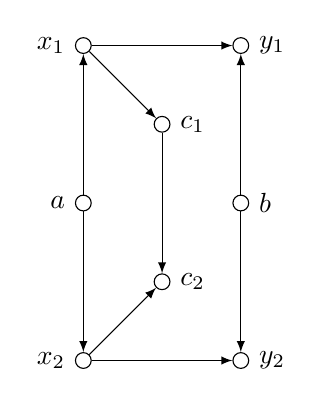
\begin{tikzpicture}
    [
    point/.style={circle,draw,inner sep=0pt,minimum size=2mm}
    ]
    \node (a) at (0,2) [point,label=left:$a$] {};
    \node (x1) at (0,4) [point,label=left:$x_1$] {};
    \node (x2) at (0,0) [point,label=left:$x_2$] {};
    \node (b) at (2,2) [point,label=right:$b$] {};
    \node (y1) at (2,4) [point,label=right:$y_1$] {};
    \node (y2) at (2,0) [point,label=right:$y_2$] {};
    \node (c1) at (1,3) [point,label=right:$c_1$] {};
    \node (c2) at (1,1) [point,label=right:$c_2$] {};
    \draw [-latex] (a) to (x1);
    \draw [-latex] (a) to (x2);
    \draw [-latex] (b) to (y1);
    \draw [-latex] (b) to (y2);
    \draw [-latex] (x1) to (y1);
    \draw [-latex] (x1) to (c1);
    \draw [-latex] (x2) to (y2);
    \draw [-latex] (x2) to (c2);
    \draw [-latex] (c1) to (c2);
  \end{tikzpicture}
  \caption{}
  \label{fig:open_door}
\end{figure}
\FloatBarrier
As before, the vertices $y_1$, $y_2$ and $c_2$ are initial vertices of disjoint rays, and not sinks.

The NAND-clause we show not to be binary-provable is $\ol{ab}$.
Figure~\ref{fig:v3_counter_proof} proves $\ol{ab}$, but the proof contains two non-binary NAND-clauses.
We will show that this is unavoidable.
In order to do this, we utilize the table from Figure~\ref{fig:v3_counter_table}.
We show it again here for convenience.\par
\begin{figure}[!h]
  \centering
  \[\begin{array}{|c||c|c|c|c|c|c|c|c|}
    \hline
    & a & b & x_1 & x_2 & y_1 & y_2 & c_1 & c_2 \\ \hline\hline
    a & \alpha_1 & & & & \alpha_1 & \alpha_1 & \alpha_1 & \alpha_2 \\ \hline
    b &-& \alpha_4 & \alpha_4 & \alpha_3 & & & \alpha_3 & \alpha_4 \\ \hline
    x_1 &-&-& \alpha_4 & & & \alpha_6 & & \alpha_6 \\ \hline
    x_2 &-&-&-& \alpha_5 & \alpha_5 & & \alpha_5 & \\ \hline
    y_1 &-&-&-&-& \alpha_1 & \alpha_1 & \alpha_1 & \alpha_2 \\ \hline
    y_2 &-&-&-&-&-& \alpha_1 & \alpha_1 & \alpha_2 \\ \hline
    c_1 &-&-&-&-&-&-& \alpha_1 & \\ \hline
    c_2 &-&-&-&-&-&-&-& \alpha_4 \\ \hline
  \end{array}\]
  \caption{}
  \label{fig:open_door_table}
\end{figure}

Suppose there is a rule application with all binary NAND-clauses in the premise and with $\ol{ab}$ in the conclusion.
Based on the (Rneg)-rule, we know that the premise must contain at least one binary NAND-clause containing $a$ and at least one containing $b$.
The above table tells us that the only provable binary NAND-clauses that contain $a$ or $b$ are the ones in the axiom set:
$\ol{ax_1}$, $\ol{ax_2}$, $\ol{by_1}$ and $\ol{by_2}$.
Since we do not want any $x_i$ or $y_i$ in the conclusion, these variables have to be removed by the OR-clause.
The OR-clauses $x_1y_1c_1$ and $x_2y_2c_2$ are the only ones that contain both an $x$ and a $y$, making them the only OR-clauses that can potentially conclude with $\ol{ab}$.

This gives us the following information: since both the possible OR-clauses are of length 3, the rule application concluding with $\ol{ab}$ has 3 NAND-clauses in its premise; one containing an $x$-vertex (either $x_1$ or $x_2$), one containing a $y$-vertex and one containing a $c$-vertex.
Looking at our table again, we see that the potentially provable NAND-clauses containing a $c$-vertex are again the axioms only.
Since there are no provable NAND-clauses on the form $ac_i$ or $bc_i$, we get that the conclusion of our rule cannot possibly be of length 2, contradicting our assumption.
We can therefore conclude that $\ol{ab}$ is \textit{not} binary-derivable, thus disproving Conjecture~\ref{thm:non_binary_derivable}.
